
% !TeX spellcheck = en_US
\documentclass{article}
\usepackage[english]{babel}
\usepackage[utf8]{inputenc}
\usepackage{fancyhdr}
\usepackage{xcolor}
\usepackage{lmodern}
\usepackage{listings}
\usepackage{amsmath}
\usepackage{amssymb}
\usepackage{graphicx}
\usepackage{physics}
\lstset{language=[90]Fortran,
	basicstyle=\ttfamily,
	keywordstyle=\color{blue},
	commentstyle=\color{green},
	morecomment=[l]{!\ }% Comment only with space after !
}

\usepackage{color}
\definecolor{deepblue}{rgb}{0,0,0.5}
\definecolor{deepred}{rgb}{0.6,0,0}
\definecolor{deepgreen}{rgb}{0,0.5,0}

% Default fixed font does not support bold face
\DeclareFixedFont{\ttb}{T1}{txtt}{bx}{n}{10} % for bold
\DeclareFixedFont{\ttm}{T1}{txtt}{m}{n}{10}  % for normal

% Python style for highlighting
\lstset{
	language=Python,
	basicstyle=\ttm,
	otherkeywords={self},             % Add keywords here
	keywordstyle=\ttb\color{deepblue},
	emph={__init__},          % Custom highlighting
	emphstyle=\ttb\color{deepred},    % Custom highlighting style
	stringstyle=\color{deepgreen},
	frame=tb,                         % Any extra options here
	showstringspaces=false            % 
}





\pagestyle{fancy}
\fancyhf{}
\lhead{Vincenzo Maria Schimmenti - 1204565}
\rhead{\today}
\rfoot{Page \thepage}
\lfoot{Exercise 8}
\title{%
	Information Theory and Computation \\
	Exercise  8}
\author{Vincenzo Maria Schimmenti - 1204565}
\begin{document}
\maketitle
 
\section*{Theory}
In this exercise we are gonna study some structures and methods in order to handle numerically pure $N$ body wavefunctions. We assume that all single particles wavefunctions $\psi_i$ live inside a $d$ dimensional Hilbert space $\mathbb{C}^d$. Hence the Hilbert space of any $N$ body wavefunction $\Psi$ is $\mathbb{C}^d \otimes \dots \otimes \mathbb{C}^d \cong \mathbb{C}^{d^N}$; a generic state of this kind can be written using single particle basis $\{ \ket{\alpha_i}, \alpha_i=0, \dots, d-1\}$:
\begin{equation}
	\Psi = \sum_{\alpha_1, \alpha_2, \dots, \alpha_N} C_{\alpha_1, \alpha_2, \dots, \alpha_N} \ket{\alpha_1} \otimes \ket{\alpha_2} \otimes \dots \otimes \ket{\alpha_N}
\end{equation}
Having chosen the basis, any wavefunction needs $d^N$ complex number to be fully specified (up to a phase). However sometimes we deal with special kinds of states, called \textit{separable}, which require only $dN$ complex coefficents and are represented as following:
\begin{equation}
	\Psi = \bigotimes_{i=1}^N \sum_{\alpha_i} C_{i, \alpha_i} \ket{\alpha_i}
\end{equation}
This kind of states are extremely important since are the basic ingredient for doing mean field theories. \\
We are also gonna study density matrices of pure states, $\rho=\ket{\Psi} \bra{\Psi}$, and ways to perform operations on them, such as traces.
\newpage
\section*{Code Development}
To encode the $N$ body pure wave function we chose to introduce a type, \textit{pstate}:
\begin{lstlisting}[language=Fortran]
type pstate
	! Hilbert space dimension
	integer*4 :: dim
	! Number of particles
	integer*4 :: np
	! Separable state
	logical :: sep
	! Wave function coefficents (either dim*np or dim**np)
	complex*16, dimension(:), allocatable :: psi
end type
\end{lstlisting}
The easiest $N$ body states to handle, as we said, is a pure separable state which needs just $dN$ coefficents, can be either represented using a $dN$ $\mathbb{C}$-vector or a $d \times N$ matrix; we chose to follow the first way with the natural convention that every $d$ coefficents in the vector we find a one particle state. If one wants to get the coefficent of the basis element $\ket{\alpha_1 \alpha_2 \dots \alpha_N}$ (where we omitted the tensor product) we can use the following code:
\begin{lstlisting}[language=Fortran]
coeff = 1.0
do ii=0,N-1
	coeff = coeff*state%psi(ii*d+sIndex(ii+1)+1)
end do
\end{lstlisting}
In the code $\textit{sIndex}$ is an integer vector containing the values of $\alpha_i, i=1\dots N$. From this implementation we understand that the method to get a $N$ body coefficient has a complexity $O(N)$. \\
The matter is more complex for indexing generic pure states; indeed we need to construct a map from all possible $\alpha_1, \dots, \alpha_N$ and an integer number that goes from $1$ to $d^N$ which spans all the basis elements. The way to do this is to use the following map:
\begin{equation}
	\text{state index}=f(\alpha_1, \dots, \alpha_N)=\alpha_1+d \alpha_2 + \dots + \alpha_N d^{N-1} = \sum_{i=1}^N d^{i-1} \alpha_i
\end{equation}
So if we start from a set of coefficents $\alpha_1, \dots, \alpha_N$ the method to retrieve the index has complexity $O(N)$:
\begin{lstlisting}[language=Fortran]
accum=1
do ii=1, N
	jj = jj + accum*sIndex(ii)
	accum = accum*d
end do
coeff = state%psi(jj+1)
\end{lstlisting}
If one wants to find all the indices of the states with a definite value $\alpha_s^*$ of the $s$-th particle one has to loop through two numbers, $r=0 \dots d^{s-1}$ and $l=0, \dots, d^{N-s}$ and build the index as $(l \times d + \alpha_s^*)d^{s-1} + r + 1$: this result is pretty useful when one wants to trace out a subsystem from a density matrix.\\
Now, given a pure state, if one wants to build a density matrix out of it, we use the following function which exploits the \textit{matmul} function of Fortran:
\begin{small}
\begin{lstlisting}[language=Fortran]
! Performs the outer product between the vector 'x' and 'y'.
! The 'y' is conjugated.
function vector_oproduct(x,y)result(rho)
	complex*16, dimension(:), intent(in) :: x,y
	complex*16, dimension(:,:), allocatable :: rho
	integer*4 :: nn, mm
	nn = size(x)
	mm = size(y)
	rho = matmul(reshape(x, (/nn,1/)), reshape(conjg(y), (/1,mm/)))
end function
\end{lstlisting}
\end{small}
Assuming the density matrix we are dealing with is build from a pure state described above, for tracing out the subsystem \textit{sSystem}:
\begin{small}
\begin{lstlisting}[language=Fortran]
sz = dd**nn
szp = dd**(nn-1)
rightMax = dd**(sSystem-1)
leftMax = dd**(nn-sSystem)
allocate(rhop(szp, szp))
factor = dd**(sSystem-1)
do rri=0, rightMax-1
	do lli=0, leftMax-1
		do rrj=0, rightMax-1
			do llj =0, leftMax-1
				! index for the traced matrix
				iip = lli*factor+rri+1
				jjp = llj*factor+rrj+1
				temp = complex(0.0,0.0)
				do val=0,dd-1
					! indices for the original matrix
					ii =(lli*dd+val)*factor+rri+1
					jj =(llj*dd+val)*factor+rrj+1
					temp = temp+rho(ii,jj)
				end do
				rhop(iip,jjp)=temp
			end do
		end do
	end do
end do
\end{lstlisting}
\end{small}
Here \textit{dd} is the Hilbert space dimension, $\textit{nn}$ the number of particles, \textit{rho} the density matrix and \textit{rhop} the resulting density matrix. 
\section*{Results}
We tried to generate different states for various number of particles (and a $2$ dimensional Hilbert space). The maximum number of particles we could acheive is $N=12$, since for bigger $N$'s Fortran could not allocate memory. \\
Using $N=2$, we tested our program both on a density matrix generated from two separable states and one explicitly given:
\begin{center}
\begin{figure}[h!]
	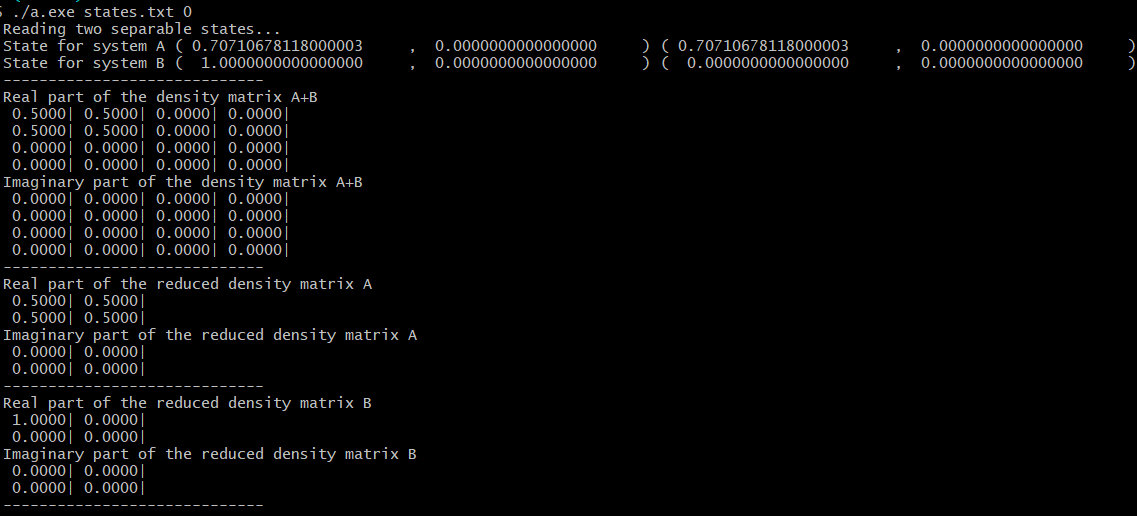
\includegraphics[width=0.85\linewidth]{sepstates.png}
\end{figure}
\begin{figure}[h!]
	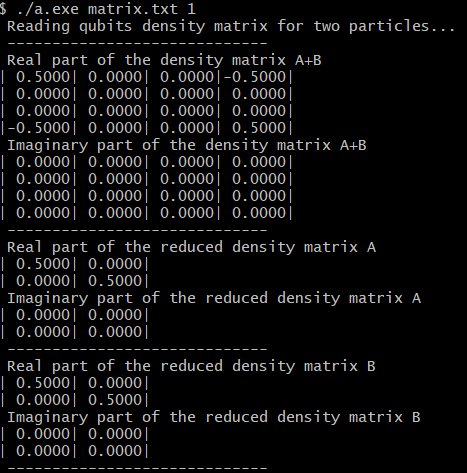
\includegraphics[width=0.5\linewidth]{matrix.png}
\end{figure}
\end{center}
The resulting density matrix are computed using the aforementioned method. For a consistency check, the first state is build from the separable state
\begin{equation}
	\left(\frac{1}{\sqrt{2}}\ket{0}_A + \frac{1}{\sqrt{2}} \ket{1}_A \right) \otimes \ket{0}_B
\end{equation}
which gives:
\begin{equation}
	\rho = \left(
	\begin{array}{cccc}
	\frac{1}{2} & \frac{1}{2} & 0 & 0 \\ 
	\frac{1}{2} & \frac{1}{2} & 0 & 0 \\ 
	0 & 0 & 0 & 0 \\ 
	0 & 0 & 0 & 0
	\end{array} 
	\right)
\end{equation}
The second is generated from:
\begin{equation}
	\frac{1}{\sqrt{2}} \ket{00} - \frac{1}{\sqrt{2}} \ket{11}
\end{equation}
i.e.:
\begin{equation}
	\rho = \left(
	\begin{array}{cccc}
	\frac{1}{2} & 0 & 0 & -\frac{1}{2} \\ 
	0 & 0 & 0 & 0 \\ 
	0 & 0 & 0 & 0 \\ 
	-\frac{1}{2} & 0 & 0 & \frac{1}{2}
	\end{array} 
	\right)
\end{equation}
\end{document}